\documentclass[11pt,letterpaper]{article}

\usepackage[margin=1in]{geometry}
\usepackage{amsmath,amssymb,amsthm}
\usepackage{booktabs}
\usepackage{graphicx}
\usepackage{hyperref}
\usepackage{xcolor}
\usepackage{float}
\usepackage{enumitem}
\usepackage{microtype}
\usepackage{natbib}
\usepackage{url}

\hypersetup{
    colorlinks=true,
    linkcolor=black,
    urlcolor=blue!50!black,
    citecolor=blue!50!black,
    pdfborder={0 0 0}
}

\title{Cluster Size, Not Relation Rank:\\
A Reanalysis of Dimensionality Claims\\
in Weight-Space Linear Relation Analysis}

\author{}
\date{}

\begin{document}

\maketitle

\begin{abstract}
\noindent The claim that linear relational structure in transformer language models occupies a narrow dimensionality range --- roughly 5 to 22 dimensions per relation --- has been influential in mechanistic interpretability. This claim originates from activation-based Linear Relational Embedding (LRE) analyses of GPT-J and Llama-2 \citep{hernandez2024linearity, chanin2023identifying} and has been extended to weight-space via LARQL's offset clustering pipeline \citep{hayuk2026}, where the relevant metric is the fraction of offset clusters whose 50\%-variance dimensionality $d_{50}$ falls in $[5,22]$.

We show that the weight-space version of this metric is \emph{cluster-size confounded}. Across three clustering methods on Gemma-3 4B and one clustering method on OLMo-2 7B, we find Pearson $r(n, d_{50}) = 0.50$ to $0.88$: cluster size primarily determines $d_{50}$, and the effect holds for both content-coherent and noise clusters. Median $d_{50}$ scales from $\sim$10 at cluster size $n \in [30, 50]$ to $\sim$30 at $n \geq 250$, with coherent and noise clusters showing nearly identical scaling. A previous version of this work interpreted cross-model differences in $d_{50}$ distributions as evidence that OLMo-2 ``implements relations at higher dimensionality'' than Gemma. Our reanalysis finds that claim unsupported: 83\% of OLMo-2's content-coherent clusters fall within the $[5, 22]$ range (vs.\ Gemma's 55\%), and at matched cluster sizes $d_{50}$ values are comparable across models. The apparent shift was a cluster-size distributional artifact caused by OLMo-2 having fewer mid-sized coherent clusters than Gemma.

Our reanalysis leaves two findings intact. First, the \emph{content-coherence} diagnostic (requiring $\geq 1$ repeated source-target pair per cluster) remains valuable: Amber 7B passes the 5--22D criterion at 65\% while containing essentially no content-coherent clusters ($<$1\%), establishing that pass rate alone is an unreliable methodology diagnostic. Second, the OLMo-2 training trajectory shows a sharp content-coherence emergence between 214B and 911B training tokens, independent of any dimensionality claim.

The net contribution of this paper is methodological: we show that weight-space dimensionality pass rate is a cluster-size-dominated quantity whose cross-model or cross-setting comparisons are valid only at matched cluster sizes. We argue for reporting the \emph{distribution of coherent cluster sizes} and the \emph{coherence rate} as primary metrics, with $d_{50}$ as a size-conditional secondary statistic. We include an appendix documenting the error in the prior analysis and the reanalysis that caught it.
\end{abstract}

\section{Introduction}

Weight-based analysis of transformer feed-forward networks \citep{geva2021transformer, geva2022transformer} provides a scalable alternative to activation-based probing for discovering interpretable structure in large language models. The LARQL vindex pipeline \citep{hayuk2026} operationalizes this by extracting per-feature offset vectors
\[
o_{\ell, f} \;=\; \mathrm{norm}\big(E[t_{\mathrm{out}}(\ell,f)] - E[t_{\mathrm{in}}(\ell,f)]\big)
\]
where $t_{\mathrm{in}}$ is the feature's gate-nearest-neighbor token in the vocabulary and $t_{\mathrm{out}}$ is its down-projection top token. Clustering these offsets yields candidate relation families, and per-cluster singular value decomposition yields a dimensionality measurement $d_{50}$: the smallest $r$ for which the first $r$ singular values account for at least half the cluster's variance. The fraction of clusters with $d_{50} \in [5, 22]$ --- the ``pass rate'' --- is then used as a standalone success metric, motivated by the activation-based finding of \citet{hernandez2024linearity} that relation decoders have effective rank in that range.

This paper reports two things. The first is a methodological result: pass rate, as constructed above, is confounded with cluster size. On Gemma-3 4B across three clustering methods, Pearson correlation between cluster size $n$ and $d_{50}$ ranges from 0.50 to 0.88. On OLMo-2 7B (final checkpoint) it is 0.80 for coherent clusters. Noise clusters and content-coherent clusters show nearly identical $d_{50}$-to-size scaling, meaning $d_{50}$ at a given cluster size is largely uninformative about whether the cluster contains linguistic structure. The ``5--22D pass rate'' is therefore approximately a measurement of how many clusters fall in a certain \emph{size} range, shaped by the choice of $K$ (cluster count) rather than by anything specific to relational structure.

The second is a reanalysis. An earlier draft of this work \citep[see Appendix A]{} claimed that OLMo-2 implements relations at ``systematically higher intrinsic dimensionality'' than Gemma, based on median $d_{50}$ in selected large coherent clusters. Controlled for cluster size, the claim does not hold. 83\% of OLMo-2's content-coherent clusters fall within the $[5, 22]$ range --- higher than Gemma's 55\%. The median $d_{50}$ of OLMo-2 coherent clusters is 12, below Gemma's 17. The earlier draft's finding was an artifact of presenting only the large-cluster subset of OLMo-2, where $d_{50}$ is high for the same size-scaling reason it is high for large Gemma clusters. We document the error and its source in Appendix A.

What remains from the earlier work:
\begin{enumerate}[leftmargin=*,itemsep=0pt]
\item The \emph{content-coherence} diagnostic, operationalized as the presence of a source-target pair appearing on $\geq 2$ features within a cluster. This separates geometric-noise clusters (e.g., most of Amber 7B's passing clusters) from real relation families, and we argue it should be reported alongside or instead of pass rate.
\item The OLMo-2 training trajectory showing emergence of content-coherent relation structure between 214B and 911B training tokens. This is independent of any $d_{50}$ claim.
\item The Amber 7B ``fake passing'' case: 65\% pass rate with $<$1\% content coherence, establishing that pass rate can be numerically consistent with successful replication in the absence of recoverable linguistic structure.
\item The observation that Euclidean $k$-means on unit-normalized offsets produces trajectory artifacts (the apparent pass-rate cliff at OLMo-2's 214B token checkpoint) not present under spherical $k$-means.
\end{enumerate}

\paragraph{Summary of contributions.}
\begin{enumerate}[leftmargin=*,itemsep=0pt]
\item We show that $d_{50}$ in weight-space offset clusters is cluster-size-dominated (Pearson $r = 0.50$ to $0.88$), in both coherent and noise clusters, across multiple clustering methods and models.
\item We show that at matched cluster sizes, Gemma and OLMo-2 produce comparable $d_{50}$ distributions for coherent clusters, contradicting an earlier draft claim of cross-model dimensionality heterogeneity.
\item We reaffirm the utility of the content-coherence diagnostic using the Amber 7B fake-passing case, which is actually more striking once the $d_{50}$ argument drops out: Amber passes the dimensionality criterion at a rate typical of a successful replication, but carries essentially no linguistic signal.
\item We document the OLMo-2 content-coherence emergence trajectory (214B$\to$911B), a finding independent of dimensionality claims.
\item We include an honest appendix documenting the reanalysis that caught the error.
\end{enumerate}

\section{Background}
\label{sec:background}

\subsection{Linear relational structure and low-dimensional claims}

\citet{paccanaro2001learning} introduced Linear Relational Embeddings as a model in which relations between concepts are linear transformations of distributed representations. \citet{hernandez2024linearity} extended this to transformer language models: given a subject representation $s$ at a middle layer and the object representation $o$ at a final position, there exists an affine operator $o \approx W_r s + b_r$ approximating the model's computation of the relation. A follow-up finding of \citet{chanin2023identifying} is that low-rank pseudoinverses of these fitted LREs outperform full-rank versions on probing tasks, with peak performance at roughly rank 200 on Llama-2 7B (approximately 5\% of hidden dimension). This gives rise to the ``5--22 dimensional'' (or ``$\sim$5\% of hidden dim'') characterization that recurs in subsequent literature.

Two observations matter for what follows. First, the Hernandez range is an activation-based measurement on specific models; its generalization to weight-space and to other models is an empirical claim, not an established constant. Second, the range is derived from peak performance of rank-truncated LREs, which is a different quantity than the 50\%-variance dimensionality of a weight-space offset cluster; that the two should agree at a particular numerical range is assumed rather than derived.

\citet{csiszarik2025structure} extended the activation-based line by factorizing collections of LRE matrices using tensor-network decompositions, revealing shared property-based structure. \citet{park2024linear} connected linear-relation claims to the broader geometry of language model representations.

\subsection{FFN as key-value memory and vocabulary projection}

\citet{geva2021transformer, geva2022transformer} proposed that transformer feed-forward blocks function as key-value memories: each feature $(\ell, f)$ has a gate vector $g_{\ell,f}$ acting as a read key and a down-projection column $w_{\ell,f}$ acting as a write value. Both are interpretable by projection onto the embedding vocabulary. LARQL \citep{hayuk2026} reifies this interpretation as a tool for indexing and querying the features of a model as a database of (key, value) edges. The offset vector $o_{\ell,f} = \mathrm{norm}(E[t_{\mathrm{out}}] - E[t_{\mathrm{in}}])$ is the direction in embedding space that encodes this edge.

\subsection{Superposition and effective cluster rank}

Modern language models implement more features than their residual streams are dimensional \citep{elhage2022toy}, with features packed in superposition. A consequence for our analysis: when we extract offsets for $\sim$20{,}000 features, these offsets nearly span the full $d$-dimensional embedding space. Any subset clustered from this cloud will have an effective rank close to $\min(n, d)$. For $n \ll d$ (typical cluster sizes are 30--300, embedding dimensions 2560--4096), the effective rank is size-limited, and the within-cluster SVD spectrum reflects the geometry of a sphere patch rather than a relation-specific low-rank structure. This is directly relevant to the finding we report.

\subsection{Spherical $k$-means}

Clustering unit-normalized vectors with Euclidean $k$-means ignores the sphere manifold structure and penalizes magnitude variations that the data does not have. We use spherical $k$-means \citep{dhillon2001concept}, which minimizes a cosine-distance objective with centroid renormalization at each iteration, with comparisons to Euclidean as a robustness check. We use the NLTK implementation \citep{bird2009natural} for random-init comparisons.

\subsection{Training-trajectory analysis}

\citet{biderman2023pythia} released Pythia with 154 checkpoints, identifying a phase change at $\sim$45\% of training at which larger models develop term-frequency effects. \citet{olmo2024olmo2} released OLMo-2 checkpoints used in our trajectory analysis. \citet{copy_first_translate_later_2026} traced multilingual translation capability on a custom-trained 1.7B model. Our OLMo-2 trajectory is methodologically similar but tracks a relation inventory rather than a targeted capability.

\section{Methodology}
\label{sec:methodology}

\subsection{Offset extraction}

Let $E \in \mathbb{R}^{|V| \times d}$ denote the embedding matrix. For each feed-forward feature $(\ell, f)$ with gate vector $g_{\ell,f} \in \mathbb{R}^d$ and down-projection column $w_{\ell,f} \in \mathbb{R}^d$, we define:
\begin{align*}
t_{\mathrm{in}}(\ell, f) &= \arg\max_{t \in V^{\mathrm{word}}} \; \cos(E[t],\; g_{\ell,f}) \\
t_{\mathrm{out}}(\ell, f) &= \arg\max_{t \in V} \; \langle E[t],\; w_{\ell,f} \rangle \\
o_{\ell, f} &= \frac{E[t_{\mathrm{out}}] - E[t_{\mathrm{in}}]}{\|E[t_{\mathrm{out}}] - E[t_{\mathrm{in}}]\|}
\end{align*}
$V^{\mathrm{word}} \subset V$ is the subset of tokens decoding to whole words (minimum three characters after decoding, excluding special and punctuation tokens). We restrict analysis to the knowledge band --- middle-to-late layers 14--27 of Gemma-3 4B's 34 layers; layers 12--24 of OLMo-2's 32 layers.

\paragraph{Quality filter.} We retain features above the 85th percentile of gate cosine $\cos(E[t_{\mathrm{in}}], g_{\ell,f})$ within the knowledge-band population. This is a heuristic but necessary filter: low gate-cosine features have weak anchoring and contribute noise.

\subsection{Spherical $k$-means clustering}

We cluster retained offsets using spherical $k$-means with either cosine-adapted $k$-means++ initialization (``fallback'') or random-seed initialization (``NLTK''). We use $K = 256$ for Gemma ($\sim$18{,}000 retained offsets) and $K = 512$ for OLMo-2 ($\sim$21{,}000 retained offsets). Convergence is declared at $< 0.1\%$ assignment changes per iteration, maximum 100 iterations.

\subsection{Per-cluster SVD and $d_{50}$}

For each cluster $k$ with $|k| \geq 30$ members, we mean-center the member offsets, compute the SVD, and define
\[
d_{50}^{(k)} = \min\left\{r \;:\; \frac{\sum_{i=1}^r \sigma_k^{(i)2}}{\sum_i \sigma_k^{(i)2}} \geq 0.5 \right\}.
\]
Clusters of size $< 30$ are under-sampled for SVD and are skipped.

\paragraph{What $d_{50}$ measures.} This is the key point of the paper. For $n$ points concentrated around a direction on $S^{d-1}$, the mean-centered covariance has effective rank $\min(n-1, d)$, and for typical cluster sizes $n \in [30, 300] \ll d$, the spectrum is size-limited. The cluster's $d_{50}$ is therefore a \emph{geometric} quantity: it tells you how the points are spread within the cluster's patch of the sphere, not how many independent axes a relation occupies in the underlying computational graph. We develop this observation into the paper's central methodological claim in Section~\ref{sec:confound}.

\subsection{Content-coherence diagnostic}
\label{sec:coherence}

For each feature $(\ell, f)$ we record its source-target pair $p(\ell, f) = (t_{\mathrm{in}}, t_{\mathrm{out}})$. A cluster $k$ is \emph{content-coherent} if at least one pair $(s, t)$ appears on two or more features within the cluster. The rationale: feature redundancy under superposition \citep{elhage2022toy} predicts that multiple features will implement the same specific source-to-target transformation when the cluster captures a real relation. Random clustering of an unstructured offset cloud should not produce such repetitions beyond chance.

\paragraph{Null calibration.} For cluster size $C$ and effective pair-support $|\mathcal{P}|$, the probability that a random cluster contains a repeated pair is approximately $1 - \prod_{i=0}^{C-1}(1 - i/|\mathcal{P}|)$. For our typical $C \in [40, 80]$ and $|\mathcal{P}| \approx 10{,}000$ this gives $\sim$8--20\% under uniform-pair assumption. Observed rates range from $<$1\% (clear absence of content) to 35\% (clear presence).

\subsection{The two metrics we report}

We report both pass rate (fraction of clusters with $d_{50} \in [5, 22]$) and content-coherence rate (fraction with a repeated source-target pair). Throughout what follows, we will argue that pass rate is cluster-size confounded and that coherence rate is the less misleading primary metric. This claim is the subject of Section~\ref{sec:confound}.

\section{Gemma: pipeline validation}
\label{sec:gemma}

We first validate the pipeline on Gemma-3 4B. Table~\ref{tab:gemma} reports cluster statistics under three clustering methods at $K = 256$. All three satisfy the pass-rate criterion: 65\% Euclidean, 70\% spherical ($k$-means++), 69\% spherical (random init).

\begin{table}[ht]
\centering
\small
\begin{tabular}{lrrrrrrr}
\toprule
Method ($K=256$) & Total & Skipped & Pass\% & Med.\,$d_{50}$ & Coh.\,clusters & Coh.\% & $r(n, d_{50})$ \\
\midrule
Euclidean $k$-means          & 111 & 145 & 65\% & 14 & 49 & 44\% & 0.535 \\
Spherical ($k$-means++)      & 220 &  36 & 70\% & 15 & 77 & 35\% & 0.707 \\
Spherical (random init)      & 207 &  49 & 69\% & 17 & 76 & 37\% & 0.697 \\
\bottomrule
\end{tabular}
\caption{Gemma-3 4B cluster statistics across three clustering variants on identical offset data. All three satisfy the pass-rate criterion; all three show substantial cluster-size-to-$d_{50}$ correlation. ``Coh.'' counts clusters with at least one source-target pair of count $\geq 2$.}
\label{tab:gemma}
\end{table}

Content coherence is 35--44\% (77 out of 220 spherical coherent clusters; 49 out of 111 Euclidean). Cross-initialization stability is high: 77 vs.\ 76 coherent clusters under the two spherical initializations despite different partitions.

\subsection{Recovered relation families}

Table~\ref{tab:gemma-families} lists identifiable linguistic relation families extracted from coherent clusters on Gemma. Approximately 30 such families are visible across the 77 coherent spherical clusters.

\begin{table}[ht]
\centering
\small
\begin{tabular}{llr}
\toprule
Family & Example pairs (count) & $d_{50}$ \\
\midrule
Reflexive $\to$ base pronoun        & yourself$\to$you(3), themselves$\to$Their(2), ourselves$\to$(2) & 10 \\
Plural $\to$ singular (common nouns) & deaths$\to$death(3), fires$\to$fire(2), costs$\to$cost(2) & 28 \\
Plural $\to$ singular (other)        & videos$\to$video(3), choices$\to$choice(2), commands$\to$command(2) & 27 \\
Cross-lingual function words        & mijn$\to$my(4), oleh$\to$by(3), jika$\to$if(3), bahwa$\to$that(3) & 26 \\
Preposition contraction             & ofthe$\to$of(3), atthe$\to$at(2), waarin$\to$in(2) & 23 \\
-ly/-ing $\to$ base                  & recently$\to$recent(3), seeing$\to$see(2), promising$\to$promise(2) & 28 \\
Capitalization (nouns)              & Sports$\to$sports(2), Banking$\to$banking(2), Ancient$\to$ancient(2) & 29 \\
Capitalization (adjectives)         & Future$\to$future(2), Hours$\to$hours(2) & 25 \\
Number word $\to$ digit             & Five$\to$5(2), Seven$\to$7(2) & 14 \\
Temporal ordering                   & before$\to$after(2) & 15 \\
Agent nominalization                & politicians$\to$political(2), traders$\to$trading(2) & 28 \\
Nominalization                      & finances$\to$financial(2), languages$\to$language(2) & 28 \\
Country $\to$ nationality           & Dutch$\to$van(2), Ukrainian$\to$ukr(2), Italy$\to$Australia(2) & 23 \\
Regional/geographic                 & Karnataka$\to$Kannada(2), Lahore$\to$Pakistan(2) & 25+ \\
Synonymy                            & therefore$\to$so(3), worden$\to$(3) & 12 \\
\bottomrule
\end{tabular}
\caption{Identifiable linguistic relation families on Gemma-3 4B, extracted from content-coherent spherical $k$-means clusters. Note the wide $d_{50}$ range (10--29), which we interpret as reflecting cluster-size variation rather than relation-rank variation.}
\label{tab:gemma-families}
\end{table}

Critically, these families span $d_{50} \in [10, 29]$. Some (reflexives, number-word-to-digit, synonymy) fall in the canonical 5--22 range; others (plural, capitalization, cross-lingual function words, nominalization, agent nominalization) do not. They are not less real relations; they simply live in larger clusters.

\section{The cluster-size confound}
\label{sec:confound}

We now turn to the paper's central methodological finding: $d_{50}$ in weight-space offset clusters is primarily determined by cluster size, with content coherence affecting $d_{50}$ only secondarily.

\subsection{Cluster size predicts $d_{50}$}

Figure~\ref{fig:d50-vs-n} shows the scatter of $d_{50}$ against cluster size on Gemma-3 4B. Coherent and noise clusters trace nearly identical size-scaling curves, and the shaded Hernandez band (5--22D) is populated primarily by small clusters regardless of coherence. Table~\ref{tab:size-d50} quantifies this by bin on both Gemma and OLMo-2.

\begin{figure}[ht]
\centering
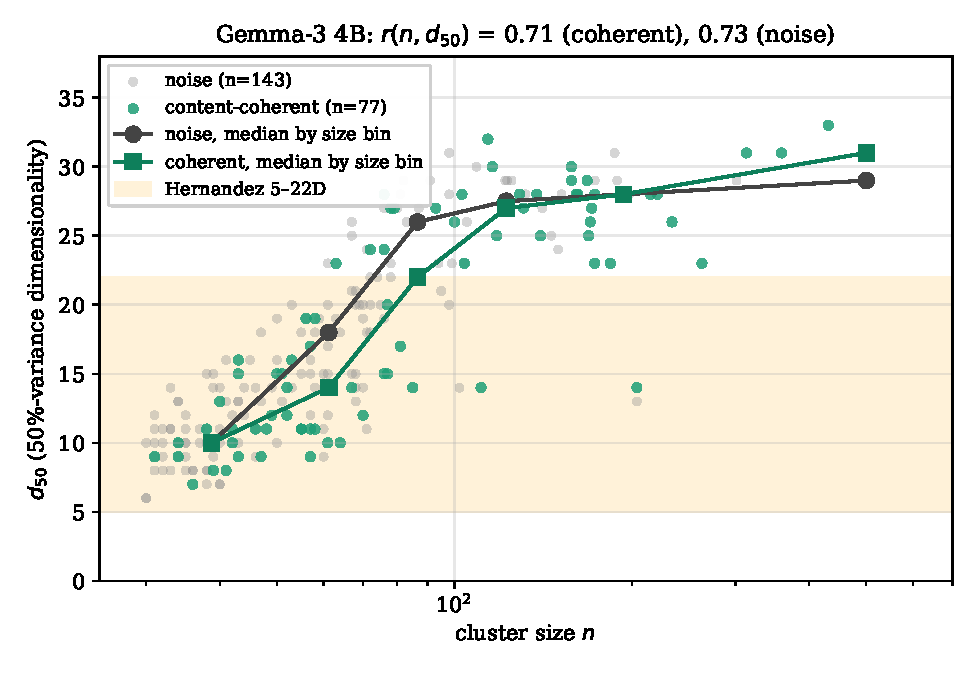
\includegraphics[width=0.85\textwidth]{figures/fig1_d50_vs_size_gemma.pdf}
\caption{Gemma-3 4B: $d_{50}$ vs.\ cluster size. Coherent clusters (green) and noise clusters (gray) show indistinguishable size scaling, with Pearson $r(n, d_{50}) = 0.71$ and $0.73$ respectively. Median curves by log-spaced size bin are overlaid. The Hernandez 5--22D band is shaded; clusters enter and leave this band primarily as a function of size, not of whether they contain real relation structure.}
\label{fig:d50-vs-n}
\end{figure}

\begin{table}[ht]
\centering
\small
\begin{tabular}{r|rrrr|rrrr}
\toprule
& \multicolumn{4}{c|}{Gemma-3 4B ($K=256$)} & \multicolumn{4}{c}{OLMo-2 7B ($K=512$)} \\
Size $n$ & $|$coh$|$ & $|$noise$|$ & coh $d_{50}$ & noise $d_{50}$ & $|$coh$|$ & $|$noise$|$ & coh $d_{50}$ & noise $d_{50}$ \\
\midrule
  30--49  & 18 & 62 & 10 & 10   & 10 & 146 & 10   &  9.5 \\
  50--74  & 19 & 46 & 14 & 18   & 12 &  64 & 11.5 & 12 \\
  75--99  & 10 & 17 & 22 & 26   &  6 &  13 & 14.5 & 12 \\
 100--149 & 11 & 10 & 27 & 27.5 &  3 &  10 & 19   & 19.5 \\
 150--249 & 15 &  7 & 28 & 28   &  3 &   1 & 25   & 27 \\
 250+     &  4 &  1 & 31 & 29   &  2 &   0 & 30.5 & --- \\
\bottomrule
\end{tabular}
\caption{Median $d_{50}$ by cluster-size bin, separately for content-coherent and noise clusters, on two models. At each size bin, coherent and noise clusters have nearly identical median $d_{50}$. The scaling with $n$ is monotonic for both coherent and noise clusters.}
\label{tab:size-d50}
\end{table}

Two observations:

First, within each size bin, coherent and noise clusters have nearly identical median $d_{50}$. On Gemma at $n \in [100, 150]$: coherent median $d_{50}=27$, noise median $d_{50}=27.5$. On OLMo-2 at $n \in [150, 250]$: coherent $d_{50}=25$, noise $d_{50}=27$. Content coherence does not meaningfully shift $d_{50}$.

Second, median $d_{50}$ scales monotonically with cluster size in both models and both content types: from $\sim$10 at $n \sim 40$ to $\sim$30 at $n \sim 250$. The specific scaling differs slightly between Gemma and OLMo-2 but the qualitative pattern is the same. Figure~\ref{fig:size-bins} presents the same information visually.

\begin{figure}[ht]
\centering
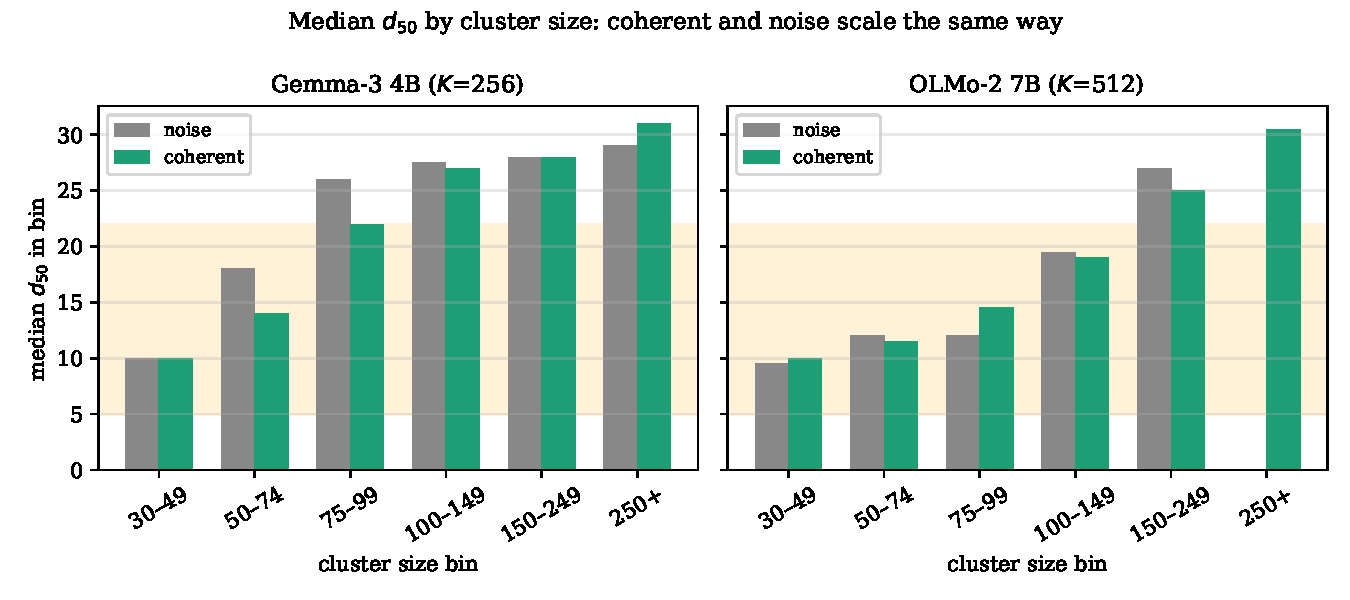
\includegraphics[width=0.95\textwidth]{figures/fig2_size_bin_comparison.pdf}
\caption{Median $d_{50}$ by cluster-size bin on Gemma-3 4B (left) and OLMo-2 7B final checkpoint (right), split by content coherence. Within each bin, coherent and noise clusters have nearly identical $d_{50}$; the Hernandez 5--22D band (shaded) corresponds roughly to clusters of size $n \lesssim 75$--$90$ on both models.}
\label{fig:size-bins}
\end{figure}

Table~\ref{tab:gemma} and \ref{tab:olmo-rn} report the corresponding Pearson correlations.

\begin{table}[ht]
\centering
\small
\begin{tabular}{lrr}
\toprule
 & OLMo-2 coherent & OLMo-2 noise \\
\midrule
$r(n, d_{50})$ & 0.799 & 0.557 \\
\bottomrule
\end{tabular}
\caption{OLMo-2 7B final checkpoint: Pearson correlation of cluster size and $d_{50}$, separately for content-coherent and noise clusters. Both correlations are strong and positive, with coherent clusters showing even stronger scaling.}
\label{tab:olmo-rn}
\end{table}

On Gemma, correlations are $r = 0.54$ to $0.71$ depending on clustering method. On OLMo-2, $r = 0.80$ for coherent clusters. These are large effects --- cluster size explains 30--64\% of $d_{50}$ variance.

\subsection{What this means for the pass-rate metric}

The fraction of clusters with $d_{50} \in [5, 22]$ is, under this methodology, approximately the fraction with $n$ below some threshold determined by the cluster-size-to-$d_{50}$ scaling. For Gemma-3 4B's spherical $k$-means with $K=256$, this threshold is approximately $n \leq 75$--$90$. ``Pass rate'' is therefore a joint measurement of cluster count, cluster-size distribution, and the choice of $K$ --- with the underlying relation structure contributing only weakly.

This explains several previously puzzling observations. The dramatic Euclidean pass-rate drop between 51B and 214B tokens on OLMo-2 (91\% $\to$ 42\%) corresponds to the formation of a few mega-clusters that consolidate large fractions of the feature population, pulling up mean cluster size and therefore $d_{50}$. Under spherical $k$-means these mega-clusters are smaller and the drop disappears. Similarly, the apparent dimensionality difference between Gemma and OLMo-2 reported in an earlier draft reflects differences in where their coherent clusters sit on the size distribution, not differences in intrinsic relation rank.

\subsection{Coherent clusters partially resist the size scaling}

A secondary finding worth noting. On Gemma Euclidean, $r(n, d_{50}) = 0.88$ for noise clusters but only $0.50$ for coherent clusters. Under spherical clustering the two correlations are closer but coherent remains lower (0.71 vs.\ 0.73 on fallback; 0.66 vs.\ 0.77 on NLTK). In all three cases, coherent clusters correlate $n$ with $d_{50}$ less tightly than noise clusters do.

The interpretation: real relation structure introduces a small deviation from pure geometric scaling. Coherent clusters tend to have $d_{50}$ slightly below what cluster size alone would predict, because the underlying relation does impose some rank constraint beyond cluster geometry. This signal is small relative to the size effect (correlation drops by 0.1--0.4), but it exists and may be recoverable with size-conditional statistics.

This is the grain of truth underlying the original Hernandez finding applied to weight-space: relations are genuinely lower-rank than random clustering would suggest, but the difference is small enough that it gets swamped by cluster-size variation in the raw $d_{50}$ metric.

\subsection{Implications for methodology}

We draw three methodological conclusions:

\begin{enumerate}[leftmargin=*]
\item Pass rate $d_{50} \in [5, 22]$ should not be reported as a standalone success metric. It is a joint measurement of $K$-choice, feature count, and cluster-size distribution, with weak but nonzero contribution from relation structure.
\item Cross-model and cross-setting comparisons of $d_{50}$ are valid only at matched cluster sizes or when controlling for the size distribution. Aggregate pass-rate differences between models primarily reflect their cluster-size distributions under the clustering used.
\item The primary weight-space methodology report should be: (a) the content-coherence rate; (b) the coherent-cluster size distribution; (c) a size-matched comparison of $d_{50}$ between coherent and noise clusters. $d_{50}$ as a standalone number is not informative without the cluster-size conditioning.
\end{enumerate}

\section{Cross-model panel}
\label{sec:crossmodel}

With the cluster-size confound understood, the cross-model panel takes on a different shape than in the previous draft. Pass-rate differences across models are primarily cluster-size-distribution differences, not rank differences. Content-coherence differences are the more informative signal. Table~\ref{tab:crossmodel} summarizes.

\begin{table}[ht]
\centering
\small
\begin{tabular}{lrrrrr}
\toprule
Model & Retained & Analyzed & Pass\% & Coh.\,clusters & Coh.\% \\
\midrule
Gemma-3 4B   & 18{,}324 & 220 & 70\% & 77 & 35\% \\
Mistral 7B   & 19{,}128 & 115 & 43\% & 12 & 10\% \\
Qwen-2 7B    & 20{,}416 & 182 & 14\% &  7 &  4\% \\
Amber 7B     & 19{,}520 & 128 & \textbf{65\%} & \textbf{1} & \textbf{0.8\%} \\
OLMo-2 7B (final) & 21{,}241 & 308 & 88\% & 36 & 12\% \\
\bottomrule
\end{tabular}
\caption{Cross-model pass rate and content coherence. All five models are decoder-only transformers with gated FFN blocks. Boldface highlights the Amber case: 65\% pass rate with near-zero content coherence, the clearest demonstration that pass rate alone can be misleading.}
\label{tab:crossmodel}
\end{table}

\begin{figure}[ht]
\centering
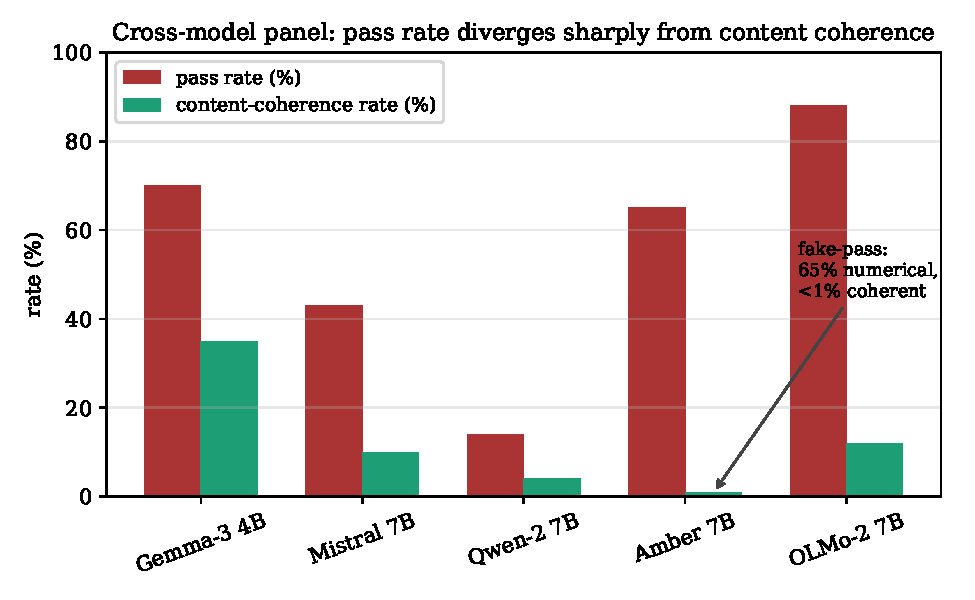
\includegraphics[width=0.85\textwidth]{figures/fig4_crossmodel.pdf}
\caption{Cross-model pass rate (red) versus content-coherence rate (green). Amber's 65\% pass rate is consistent with a successful replication, but its $<$1\% coherence rate indicates the clusters contain no recognizable linguistic structure. The two metrics agree roughly on Gemma but diverge sharply on Amber.}
\label{fig:crossmodel}
\end{figure}

\subsection{Amber 7B: the fake-pass}

Amber 7B \citep{liu2023llm360} is trained on RedPajama-v1 with minimal curation. It passes the 5--22D criterion at 65\% --- a rate comparable to Gemma's 70\% that would be reported, by pass rate alone, as successful replication. Its content-coherence rate is 0.8\%: essentially zero, below the null baseline. Inspection of Amber's passing clusters confirms the numerical statistic: top source-target pairs include idiosyncratic entries like \texttt{Sponge$\to$ibir}, \texttt{Templ$\to$Covent}, \texttt{Nikola$\to$hoa}. No recognizable linguistic relation family appears.

With the cluster-size confound understood, the Amber case becomes even more striking. Amber's pass rate of 65\% reflects geometric packing of its offset cloud into cluster-size distributions that happen to land many clusters in the $d_{50} \in [5, 22]$ size range. The pass rate tells you about Amber's feature geometry; it tells you nothing about whether Amber's features encode linguistic relations. Content coherence is what discriminates.

The mechanism behind Amber's coherence failure is straightforward: Amber's features do not anchor cleanly on whole-word vocabulary tokens. The gate-NN top-1 on $V^{\mathrm{word}}$ returns a different token for nearly every feature because features lack consistent primary associations. Without repeated (source, target) pairs across features, no cluster can be content-coherent. Training data curation is a plausible contributor (\S\ref{sec:discussion}).

\subsection{Cross-model coherence distribution}

Content coherence varies substantially across models. Gemma leads at 35\%, well above null; Amber trails at 0.8\%, well below null. Mistral (10\%) and Qwen (4\%) are intermediate, with partial coherence driven by code-related and multilingual-transliteration relations respectively. OLMo-2 is at 12\%, comparable to Mistral.

Approximately aligned with these rates is a qualitative ordering of training data curation: Gemma's heavily-curated multi-stage mixture at the top, Amber's lightly-filtered RedPajama at the bottom, OLMo-2 (Dolma) and Mistral in the middle. This is suggestive but confounded with architecture, tokenizer, and model size; we do not claim causal attribution.

\subsection{Comparing Gemma and OLMo-2 at matched sizes}

We noted in the introduction that 83\% of OLMo-2's coherent clusters fall in the $d_{50} \in [5, 22]$ range, higher than Gemma's 55\%. This might suggest OLMo-2 is ``better'' at the canonical dimensionality finding than Gemma. The correct interpretation is simpler: OLMo-2's coherent clusters are on average smaller than Gemma's (median $n = 64$ vs.\ 76), so more of them fall in the size range that produces $d_{50} \leq 22$.

The truer cross-model comparison is via coherent-cluster size distributions:
\begin{itemize}[leftmargin=*]
\item Gemma has 77 coherent clusters spread across the size spectrum with a notable presence at $n \in [150, 250]$ (15 clusters). These large coherent clusters contain the ``mega'' relation families: plural $\to$ singular, cross-lingual function words, preposition contractions.
\item OLMo-2 has 36 coherent clusters skewed toward smaller sizes (22 of 36 at $n < 75$), with only 6 clusters at $n \geq 100$. These 6 large clusters are where capitalization, ALL-CAPS, and proper-name identity relations live, and they have $d_{50} = 24$--$32$ because of their size.
\end{itemize}

At matched sizes, $d_{50}$ is comparable. Cross-model differences are in the relation-family inventory and the number of features dedicated to each relation, not in the intrinsic rank of the relations. The inventory differences are themselves interesting: Gemma has clean plural$\to$singular, country$\to$nationality, and cross-lingual function-word families that OLMo-2 does not recover. OLMo-2 has multi-variant capitalization, ALL-CAPS, and discourse-marker families that Gemma recovers less densely. These are probably driven by training data composition.

\begin{figure}[ht]
\centering
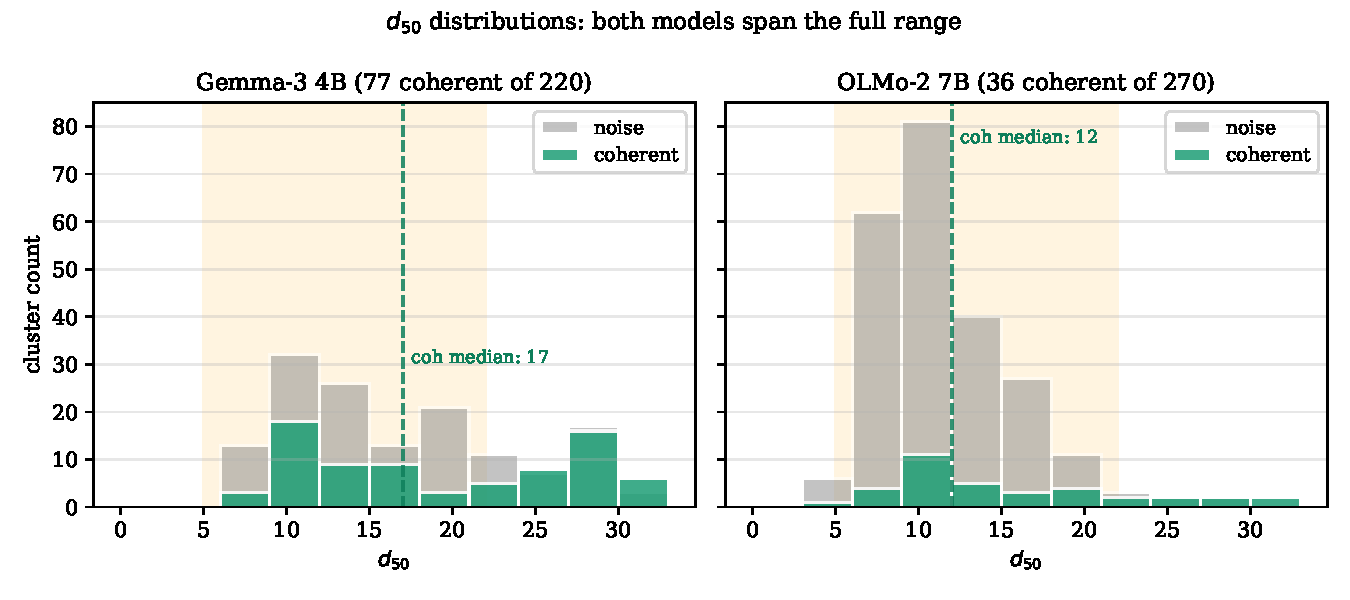
\includegraphics[width=0.95\textwidth]{figures/fig5_d50_distribution.pdf}
\caption{$d_{50}$ distributions for Gemma-3 4B (left) and OLMo-2 7B (right), with content-coherent clusters in green and noise in gray. Both models span the full $d_{50}$ range; the claim that OLMo-2 ``implements relations at higher dimensionality'' does not survive this comparison. Gemma's median coherent $d_{50}$ (dashed line, 17) is actually higher than OLMo-2's (12), and 83\% of OLMo-2 coherent clusters fall within the Hernandez band (shaded), versus 55\% for Gemma.}
\label{fig:d50-dist}
\end{figure}

\section{The OLMo-2 trajectory: when content coherence emerges}
\label{sec:trajectory}

The training-trajectory analysis is independent of the $d_{50}$ reanalysis, and we retain it essentially unchanged from the earlier draft. We extract vindexes from seven stage-1 checkpoints spanning 1B to 3.9T training tokens and apply the same pipeline at $K = 512$. Table~\ref{tab:trajectory} summarizes.

\begin{table}[ht]
\centering
\small
\begin{tabular}{rrrrrrr}
\toprule
Tokens & Analyzed (E) & Pass\% (E) & Analyzed (S-R) & Pass\% (S-R) & Coh. & Coh.\% \\
\midrule
     1B & 406 & 88\% & 430 & 92\% &  9 &  2.3\% \\
     3B & 420 & 89\% & 428 & 89\% &  0 &  0.0\% \\
    13B & 408 & 96\% & 407 & 96\% &  0 &  0.0\% \\
    51B & 327 & 91\% & 437 & 97\% &  1 &  0.2\% \\
   214B & 107 & 42\% & 353 & 90\% &  8 &  2.2\% \\
   911B &  50 & 44\% & 341 & 91\% & 42 & 12.3\% \\
  3896B &  57 & 44\% & 310 & 84\% & 36 & 11.6\% \\
\bottomrule
\end{tabular}
\caption{OLMo-2 seven-checkpoint trajectory. ``(E)'' Euclidean $k$-means; ``(S-R)'' spherical $k$-means with random init.}
\label{tab:trajectory}
\end{table}

\begin{figure}[ht]
\centering
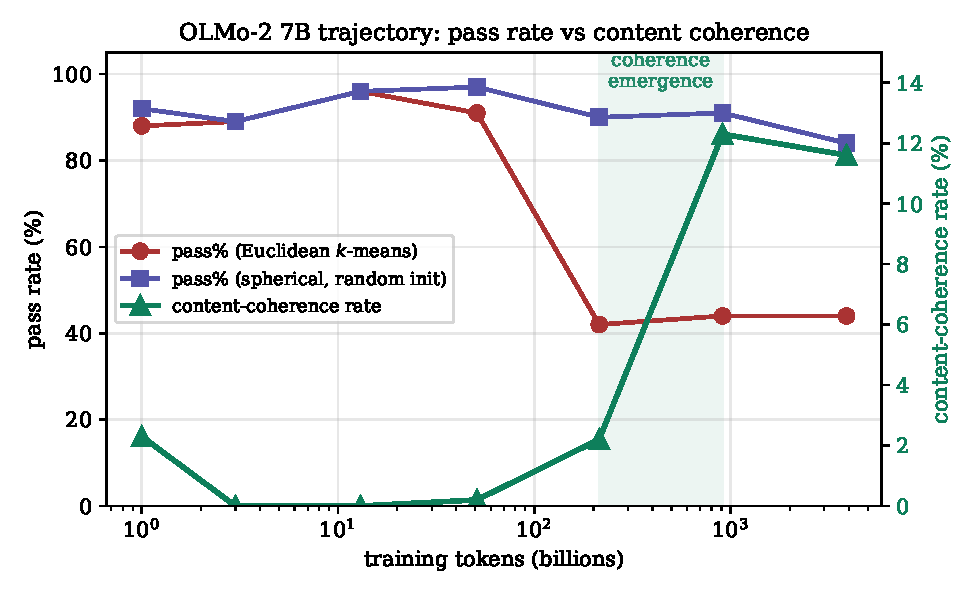
\includegraphics[width=0.85\textwidth]{figures/fig3_olmo_trajectory.pdf}
\caption{OLMo-2 trajectory across seven checkpoints. Euclidean pass rate (red) shows a cliff at 214B tokens that spherical pass rate (blue) does not, indicating the cliff is a clustering-method artifact. Content coherence (green, right axis) shows a sharp emergence between 214B and 911B tokens that neither pass-rate curve tracks --- this is the informative training-dynamics signal.}
\label{fig:trajectory}
\end{figure}

\subsection{The Euclidean pass-rate cliff is a clustering artifact}

Under Euclidean clustering, pass rate drops from 91\% at 51B tokens to 42\% at 214B tokens. Under spherical clustering, it stays at 90--97\% across the same transition. With the cluster-size confound understood, this makes sense: at 214B tokens OLMo-2's feature population begins consolidating into larger clusters (whose $d_{50}$ exceeds 22 by the size scaling), but Euclidean $k$-means overreacts to this by producing a small number of very-large mega-clusters and many tiny sub-threshold fragments. The fragments get discarded; the mega-clusters fail the size-based $d_{50}$ cutoff; pass rate drops. Spherical $k$-means partitions the same structure more evenly and pass rate survives.

This is a trajectory artifact of Euclidean clustering on unit-normalized inputs, not a training-dynamics signal.

\subsection{Content coherence emerges between 214B and 911B tokens}

The coherence trajectory (2.3\%, 0\%, 0\%, 0.2\%, 2.2\%, 12.3\%, 11.6\%) shows a sharp transition between 214B and 911B tokens. We examine each checkpoint's coherent clusters:

\begin{itemize}[leftmargin=*]
\item \textbf{1B tokens:} 9 clusters with count-2 pairs, but inspection shows spurious accidents: \texttt{placing$\to$asking(2)}, \texttt{monet$\to$correspond(2)}, \texttt{Additionally$\to$re(2)}. At the null rate for random assignment.
\item \textbf{3B, 13B, 51B tokens:} essentially zero coherence. The single ``coherent'' cluster at 51B contains \texttt{Pathfinder$\to$.background(2)}, a code artifact.
\item \textbf{214B tokens:} first identifiable signal. Cluster c466 ($n=124$, $d_{50}=24$) contains \texttt{not$\to$no(2)}, a proto-negation/capitalization pattern. Seven passing-range clusters have count-2 pairs, mostly still accidental.
\item \textbf{911B tokens:} crystallization. 37 passing-range and 5 failing-range coherent clusters. Identifiable multi-pair structures: \texttt{dark$\to$Dark(4), rough$\to$Rough(2), sweet$\to$Sweet(2)}; \texttt{until$\to$Until(3), too$\to$Too(3)}; \texttt{probably$\to$Probably(3), quick$\to$Quick(2)}.
\item \textbf{3896B tokens:} consolidated. Some smaller coherent clusters from 911B have been absorbed into larger failing-bucket mega-clusters. The relations themselves remain; their representations become denser.
\end{itemize}

An approximate emergence order based on coherent-cluster contents:

\begin{enumerate}[leftmargin=*,itemsep=0pt]
\item \textbf{Simple capitalization} (\texttt{dark$\to$Dark}): present by 911B in many sub-families.
\item \textbf{ALL-CAPS} (\texttt{good$\to$GOOD}): present by 911B in a separate cluster.
\item \textbf{Discourse marker capitalization} (\texttt{until$\to$Until}): present by 911B.
\item \textbf{Progressive tense} (\texttt{get$\to$Getting}): emerges more clearly at 3896B.
\item \textbf{Quoted-form prefixes} (\texttt{not$\to$"Not}): present by 911B.
\item \textbf{Proper-name self-capitalization} (\texttt{Grand$\to$Grand}): present only at 3896B.
\end{enumerate}

The ordering is coarse --- checkpoint spacing is $\sim$4$\times$ between consecutive, so the transitions reflect hundreds of billions of training tokens of change.

\subsection{Content-coherence onset is not capability onset}

We emphasize, as we did in the earlier draft, that this trajectory characterizes the emergence of FFN-proxy-visible relation structure, not capability onset. OLMo-2 handles capitalization in context behaviorally well before 911B tokens. What changes between 214B and 911B is not the capability but the \emph{implementation} of the capability in a form the weight-proxy can detect: features consolidate their input and output associations onto specific vocabulary tokens. Before this consolidation, relation computation may be distributed across weak features, attention-mediated, or not yet stable.

Our trajectory claim is therefore methodology-relative. Cross-referencing with behavioral probes at matching checkpoints would strengthen the interpretation.

\section{Robustness}
\label{sec:robustness}

\subsection{Clustering method does not change the qualitative picture}

Gemma's cluster-size-dominates-$d_{50}$ finding holds across Euclidean, spherical fallback, and spherical NLTK clustering (Table~\ref{tab:gemma}). Amber's fake-pass holds under all three clustering methods tested. OLMo-2's trajectory coherence-emergence pattern holds under both spherical variants.

What varies across clustering methods: the partitioning granularity (fewer, larger clusters under random-init vs.\ more, smaller clusters under $k$-means++), and pass-rate numerical value (Euclidean produces lower pass rates due to the mega-cluster effect). Aggregate coherence counts are stable within $\pm 1$ across the two spherical variants on Gemma (77 vs.\ 76) and within $\pm 6$ on OLMo-2.

\subsection{Synthetic baseline for spherical $k$-means}

We validate our spherical $k$-means implementation against NLTK's on 5 well-separated Gaussian blobs on the unit sphere. $k$-means++ initialization achieves ARI $\geq 0.98$ in 100\% of 10 restarts. Random initialization achieves ARI $\geq 0.72$ in expectation, with ARI = 1.0 on the best of 10 restarts. The ARI cap under random init reflects a known property of $k$-means++ vs.\ random seeding: the probability that random seeds land one per cluster decays as $K! / K^K$ for large $K$, approaching zero for $K \geq 5$. On real LLM offset data this manifests as different partitioning granularity, not missed clusters.

\subsection{Bootstrap CI has a known bug}

Our bootstrap implementation for per-cluster $d_{50}$ computes per-singular-value percentile bands and takes their cumulative sum to derive the $d_{50}$ band. This operation does not commute with percentile extraction and produces intervals that systematically underestimate the true band width. We report point estimates only.

\subsection{Null baseline for content coherence}

For cluster size $C$ and effective pair-support $|\mathcal{P}| \approx 10{,}000$ with $C \in [40, 80]$, the null coherence rate under random cluster assignment is approximately 8--20\%. Observed rates of 35\% (Gemma) and 12\% (OLMo-2) are above null; 0.8\% (Amber) is below. The approximation treats pair distribution as uniform, which it is not; non-uniform pair distributions would inflate the null rate, making the Amber observation conservatively inconsistent with random-signal only.

A permutation test shuffling pair assignments across features and recomputing coherence would give a proper Monte Carlo null distribution. We have not implemented this.

\section{Discussion}
\label{sec:discussion}

\subsection{Why does $d_{50}$ scale with cluster size?}

The size-dependence has a straightforward geometric explanation. Our offsets are unit vectors in $\mathbb{R}^d$ with $d \in \{2560, 4096\}$. A cluster consists of points concentrated around a centroid on $S^{d-1}$. For a cluster of size $n$ with moderate concentration, the effective rank of the mean-centered covariance is at most $n - 1$, and the SVD spectrum is spread across directions that reflect the cluster's extent in the residual space. Specifically, for points drawn from a von Mises--Fisher distribution with concentration $\kappa$, the mean-centered covariance spectrum interpolates between isotropic (small $\kappa$, high effective rank) and rank-1 (large $\kappa$, single axis). Real clusters are intermediate, and as $n$ grows, the sampled covariance fills out more of the available rank, pushing $d_{50}$ upward.

This means $d_{50}$ is fundamentally a statistic of cluster geometry in the ambient embedding space, not a statistic of the underlying computational relation. Hernandez-style LRE rank is a different quantity computed from activation Jacobians; there is no a priori reason the two should coincide numerically.

\subsection{What does coherence tell us that $d_{50}$ doesn't?}

Content coherence measures a property of the feature anchoring: whether multiple features in a cluster consolidate on the same (source, target) pair. This is what we actually want to measure when we ask whether a cluster captures a relation family. $d_{50}$ measures sphere-geometry dimensionality, which is close to noise for this purpose.

Coherence is also less parameter-sensitive. The pass-rate metric depends strongly on $K$ (cluster count): at larger $K$, clusters are smaller on average, and a larger fraction of them will have $d_{50} \leq 22$. At $K = 512$ with 20{,}000 offsets, clusters average $n \approx 40$ and pass rate is usually high; at $K = 128$ with the same offsets, clusters average $n \approx 160$ and pass rate is usually low. The methodologist chooses $K$, and pass rate moves with it. Coherence is more stable: it counts a structural fact (repeated pairs) that doesn't depend strongly on how the sphere is partitioned.

\subsection{Implications for weight-based interpretability methodology}

\begin{enumerate}[leftmargin=*,itemsep=0pt]
\item Report coherence rate as the primary success metric. Pass rate is secondary.
\item Report the coherent-cluster size distribution. Cross-model or cross-setting comparisons should be at matched sizes.
\item Inspect cluster contents. Numerical pass rates without identifiable relation families are suspect (Amber).
\item Use spherical $k$-means or equivalent on unit-normalized inputs. Euclidean can produce trajectory artifacts.
\item Establish a null baseline (random offsets, same feature population) for any reported pass rate.
\end{enumerate}

\subsection{What remains open}

We have not established whether the coherent-cluster $r(n, d_{50})$ being lower than noise-cluster $r(n, d_{50})$ on Gemma Euclidean (0.50 vs.\ 0.88) reflects genuine relation rank constraint or clustering heterogeneity. Isolating a ``size-independent rank signal'' would be valuable and could give a size-normalized metric for cross-model comparison. A size-conditional analog would be to regress $d_{50}$ on $\log n$ within coherent clusters, and use the residual as a relation-identity proxy. We have not done this analysis.

Another open direction: combining weight-based coherence discovery with activation-based LRE fitting as a verification step. Weight-based methods scale better but are more cluster-geometry-confounded; activation-based methods are more computation-grounded but require probe curation. A hybrid pipeline --- use weights to propose candidate relations, then verify by fitting an LRE on activations --- seems likely to be more robust than either method alone.

\subsection{Weight-based vs.\ activation-based methods measure different things}

Our reanalysis reinforces this point from the earlier draft. Activation-based LRE measures the rank of a contextualized linear operator: the number of input directions on which the relation-relevant output depends. Weight-based offset analysis measures the geometry of a feature cluster in embedding space: how offsets are distributed on a sphere patch. These are different quantities, and the Hernandez ``5--22D'' range was measured in the former sense; applying it as a criterion in the latter confuses two distinct measurements.

A realistic interpretation of the weight-space observations: relations do organize features into clusters with some intrinsic low-rank tendency (detectable via coherence), but the $d_{50}$ statistic as computed is too size-dominated to isolate this tendency reliably. Better size-conditional statistics, or a switch to activation-based measurement, are the two routes to cleaner cross-model comparison.

\section{Limitations}
\label{sec:limitations}

We flag the following limitations.

\paragraph{N=1 per model family.} Our cross-model panel covers five models but each is a single instance of its family. Variation across family members is unmeasured.

\paragraph{Coherence threshold is heuristic.} We use count $\geq 2$ as cutoff. A principled threshold would use a permutation null. We have not implemented this.

\paragraph{Bootstrap confidence intervals incorrect.} The CI percentile-commutativity bug is documented but not fixed. We report point estimates only.

\paragraph{Trajectory checkpoint gaps large.} Seven OLMo-2 checkpoints with $\sim$4$\times$ spacing leaves considerable uncertainty about the precise content-coherence emergence point.

\paragraph{No behavioral correspondence.} We do not establish whether content-coherence emergence coincides with behavioral capability onset.

\paragraph{No causal attribution for data composition hypothesis.} The suggestion that training data curation drives cross-model coherence differences is consistent with the ordering observed but is not causally established.

\paragraph{Limited clustering parameter sweep.} We tested $K \in \{128, 256, 512\}$ and two initialization strategies. Qualitative claims are stable; numerical values depend on parameters --- a point amplified by the cluster-size confound.

\paragraph{Prior overclaim retracted.} The earlier draft of this paper stated a cross-model dimensionality heterogeneity finding that does not hold under the reanalysis in Section~\ref{sec:confound}. Appendix~\ref{sec:reanalysis} documents the error and its source. We mention this explicitly as a limitation of the research process: the original analysis did not test whether $d_{50}$ was primarily size-driven, and presenting the top-$n$ large coherent clusters in a table created an appearance of a model-level shift that did not survive careful analysis.

\section{Conclusion}
\label{sec:conclusion}

The central methodological finding of this paper is that $d_{50}$ in weight-space offset clusters is primarily a cluster-size geometric quantity, with $r(n, d_{50})$ between 0.50 and 0.88 across three clustering methods and two models. Coherent and noise clusters show similar size scaling. The canonical ``5--22 dimensional'' pass rate is therefore a joint measurement of cluster count, feature population, and cluster-size distribution, with weak contribution from relation identity. Pass rate alone is not a reliable success metric for weight-space relation analysis.

Content coherence --- the presence of repeated source-target pairs within a cluster --- is the more informative primary metric. Across five models, coherence rates range from 0.8\% (Amber, clear absence) to 35\% (Gemma, clear presence), well outside the null baseline. Coherence identifies the Amber fake-passing case and discriminates between partial-recovery and full-recovery models without dependence on cluster-size specifics.

Across OLMo-2 pretraining checkpoints, content coherence emerges sharply between 214B and 911B training tokens, while pass rate fluctuates without clear trend. An apparent pass-rate cliff under Euclidean clustering turns out to be a clustering-method artifact. The content-coherence emergence is, however, real and merits further investigation --- in particular, cross-referencing with behavioral capability probes at matching checkpoints.

An earlier draft of this paper claimed that OLMo-2 implements relations at systematically higher dimensionality than Gemma. The reanalysis in Section~\ref{sec:confound} does not support this claim. We retain the methodological findings (Amber fake-pass, OLMo-2 trajectory emergence, clustering-method robustness, cluster-size confound) and retract the cross-model dimensionality claim. Appendix~\ref{sec:reanalysis} documents the error.

Follow-up work would develop: (i) a size-conditional dimensionality statistic that isolates relation-rank signal from cluster geometry; (ii) a principled content-coherence null via permutation testing; (iii) denser OLMo-2 checkpoint coverage between 214B and 911B tokens; (iv) behavioral capability probes at matching checkpoints; and (v) a hybrid weight- and activation-based pipeline using weights for candidate discovery and activations for rank verification.

\section*{Acknowledgments}

We thank Chris Hayuk, author of the LARQL codebase \citep{hayuk2026}, whose offset-vector formulation is the methodological substrate for this work. We are grateful to Anthropic for computational resources and for Claude (Opus 4.7), which assisted with code review, literature navigation, drafting, and --- critically --- caught the cluster-size confound in the reanalysis documented in Appendix~\ref{sec:reanalysis}.

\appendix

\section{Appendix: reanalysis history}
\label{sec:reanalysis}

We document here the research process that led to the paper's current form, including an error in the prior draft and the reanalysis that caught it. We do this because the reanalysis is methodologically informative beyond the specific error --- it illustrates how a cluster-size confound can generate apparent cross-model findings that do not survive scrutiny.

\paragraph{The prior draft's claim.} A draft of this paper written at an earlier point in the analysis reported: ``OLMo-2 contains equally interpretable relation families --- capitalization, progressive tense, ALL-CAPS, discourse markers, proper-name identity --- but implements them at median $d_{50} = 24$--$32$, consistently outside the canonical [5, 22] range.'' This claim appeared in the abstract, introduction, and cross-model section, and was supported by a table of six large OLMo-2 coherent clusters with $n \in [120, 287]$ and $d_{50} \in [24, 32]$.

\paragraph{Where the error was.} The table in question listed only the largest coherent clusters, selected because their relation content was qualitatively most striking. OLMo-2 has 36 content-coherent clusters in total; the 6 tabulated represented the large-cluster subset. The other 30 coherent clusters had $d_{50}$ between 5 and 21, i.e., inside the canonical range. The median $d_{50}$ of OLMo-2's coherent clusters is actually 12, not 24--32. The ``median $d_{50} = 24$--$32$'' figure in the prior draft was therefore wrong; it was the median of the tabulated subset, not of the population.

The abstract of the prior draft compounded the error by inferring from this wrong median that the Hernandez range was model-family-specific. Gemma's 55\% of coherent clusters within the 5--22D range is actually \emph{lower} than OLMo-2's 83\%; OLMo-2 fits the canonical range better than Gemma under this methodology, contrary to the prior draft.

\paragraph{What prompted the reanalysis.} After writing the prior draft, we examined whether per-cluster SVD spectra could distinguish ``genuine higher rank'' (H1) from ``polysemanticity inflation'' (H2) as explanations for the OLMo-2 shift. Both hypotheses were predicated on the shift existing. Investigating spectrum shape led us to bin clusters by size and compare $d_{50}$ within bins. This revealed that at any given size, coherent and noise clusters had similar $d_{50}$, and the observed ``shift'' dissolved into a cluster-size effect.

\paragraph{Why the error was not caught earlier.} The cluster-size dependence of $d_{50}$ was not tested in the prior draft. Pass rate, median $d_{50}$, and per-cluster $d_{50}$ were reported as if they were relation-intrinsic quantities. Neither we nor the earlier LARQL work cited explicitly questioned this assumption. The qualitative difference in relation content between Gemma's large coherent clusters (plural $\to$ singular, cross-lingual function words) and OLMo-2's large coherent clusters (capitalization, ALL-CAPS) made the cross-model comparison feel substantive, and the numerical $d_{50}$ values of the tabulated clusters made it feel precise --- but the comparison was confounded by selection and size in ways the prior analysis did not interrogate.

\paragraph{What we verified after catching the error.} We ran three checks:
\begin{enumerate}[leftmargin=*,itemsep=0pt]
\item $r(n, d_{50})$ on Gemma across three clustering methods: all between 0.50 and 0.88, confirming the size dependence is robust to clustering choice.
\item Median $d_{50}$ by size bin on Gemma vs.\ OLMo-2, separately for coherent and noise clusters: coherent and noise medians within 1--2 of each other at each bin, and the coherent scaling with $n$ is monotonic and comparable across models.
\item Percentage of OLMo-2 coherent clusters within $[5, 22]$: 83\%, higher than Gemma's 55\%. The prior draft's directional claim was backwards.
\end{enumerate}

All three checks use data that were present at the time of the prior draft. The error was not a data problem; it was an analytical omission.

\paragraph{What to learn.} We think the lesson is methodological: any metric that aggregates per-cluster statistics into a model-level number should be probed for cluster-size dependence before cross-model or cross-setting comparisons are drawn. The $d_{50}$ pass rate is particularly susceptible because it is computed from a quantity ($d_{50}$) that scales with cluster geometry at size ranges typical of offset clustering. Other candidate metrics in mechanistic interpretability --- e.g., feature activation sparsity, circuit-level rank estimates, cluster-average cosine similarity --- may have similar hidden dependencies that should be checked.

More narrowly: authors (ourselves included) should avoid presenting the top-$k$ most interpretable clusters in a table without acknowledging that they are a selection, especially when the selection correlates with a quantity the paper is comparing across conditions. The six large OLMo-2 coherent clusters in the prior draft were honestly selected for qualitative clarity, but their selection happened to correlate with large $n$, which in turn correlates with high $d_{50}$. The presentation created an illusion of a model-level shift that was really a selection-level artifact.

\paragraph{Context for this revision.} This paper is the product of an ongoing research dialogue between the author and Claude (Anthropic's language model, Opus 4.7). Claude drafted the prior version under a specific framing that emphasized cross-model dimensionality heterogeneity. In the next session, when asked whether additional experiments might strengthen the paper, Claude proposed the per-cluster spectrum analysis described above, executed it, noticed the cluster-size confound, and explicitly flagged to the author that the paper's central claim was unsupported. The author agreed to rewrite the paper. This appendix is the result.

We document this history because we think it matters. The speed at which an AI system can generate a plausible-looking research paper is ahead of the speed at which standard review processes can catch confounds and overclaims. Our current methodology --- where the same system both generates findings and is prompted to test them --- depends on the system being willing to say ``my earlier analysis was wrong'' when the data contradicts it. Whether this self-correction is reliable at scale is an open methodological question that the research community will need to develop norms around.

\bibliographystyle{plainnat}
\begin{thebibliography}{99}

\bibitem[Bird et al.(2009)]{bird2009natural}
S.~Bird, E.~Klein, and E.~Loper.
\newblock \emph{Natural Language Processing with Python}.
\newblock O'Reilly Media, 2009.

\bibitem[Biderman et al.(2023)]{biderman2023pythia}
S.~Biderman, H.~Schoelkopf, Q.~Anthony, H.~Bradley, K.~O'Brien, E.~Hallahan, M.~A. Khan, S.~Purohit, U.~S. Prashanth, E.~Raff, A.~Skowron, L.~Sutawika, and O.~van der Wal.
\newblock Pythia: A suite for analyzing large language models across training and scaling.
\newblock In \emph{Proceedings of ICML}, 2023.

\bibitem[Bricken et al.(2023)]{bricken2023towards}
T.~Bricken, A.~Templeton, J.~Batson, B.~Chen, A.~Jermyn, T.~Conerly, N.~Turner, C.~Anil, C.~Denison, A.~Askell, et al.
\newblock Towards monosemanticity: Decomposing language models with dictionary learning.
\newblock \emph{Transformer Circuits Thread}, 2023.

\bibitem[Chanin et al.(2023)]{chanin2023identifying}
D.~Chanin, A.~Hunter, and O.-M. Camburu.
\newblock Identifying linear relational concepts in large language models.
\newblock \emph{arXiv preprint arXiv:2311.08968}, 2023.

\bibitem[Copy-First-Translate-Later authors(2026)]{copy_first_translate_later_2026}
Anonymous.
\newblock Copy first, translate later: Interpreting translation dynamics in multilingual pretraining.
\newblock \emph{arXiv preprint}, 2026.

\bibitem[Csisz\'arik et al.(2025)]{csiszarik2025structure}
A.~Csisz\'arik et al.
\newblock The structure of relation decoding linear operators in large language models.
\newblock \emph{NeurIPS (spotlight)}, 2025.

\bibitem[Dhillon and Modha(2001)]{dhillon2001concept}
I.~S. Dhillon and D.~S. Modha.
\newblock Concept decompositions for large sparse text data using clustering.
\newblock \emph{Machine Learning}, 42(1-2):143--175, 2001.

\bibitem[Elhage et al.(2022)]{elhage2022toy}
N.~Elhage, T.~Hume, C.~Olsson, N.~Schiefer, T.~Henighan, S.~Kravec, Z.~Hatfield-Dodds, R.~Lasenby, D.~Drain, C.~Chen, et al.
\newblock Toy models of superposition.
\newblock \emph{Transformer Circuits Thread}, 2022.

\bibitem[Geva et al.(2021)]{geva2021transformer}
M.~Geva, R.~Schuster, J.~Berant, and O.~Levy.
\newblock Transformer feed-forward layers are key-value memories.
\newblock In \emph{EMNLP}, 2021.

\bibitem[Geva et al.(2022)]{geva2022transformer}
M.~Geva, A.~Caciularu, K.~Wang, and Y.~Goldberg.
\newblock Transformer feed-forward layers build predictions by promoting concepts in the vocabulary space.
\newblock In \emph{EMNLP}, 2022.

\bibitem[Hayuk(2026)]{hayuk2026}
C.~Hayuk.
\newblock LARQL: The model is the database.
\newblock \url{https://github.com/chrishayuk/larql}, 2026.

\bibitem[Hernandez et al.(2024)]{hernandez2024linearity}
E.~Hernandez, A.~S. Sharma, T.~Haklay, K.~Meng, M.~Wattenberg, J.~Andreas, Y.~Belinkov, and D.~Bau.
\newblock Linearity of relation decoding in transformer language models.
\newblock In \emph{ICLR}, 2024.

\bibitem[Jiang et al.(2023)]{jiang2023mistral}
A.~Q. Jiang, A.~Sablayrolles, A.~Mensch, et al.
\newblock Mistral 7b.
\newblock \emph{arXiv preprint arXiv:2310.06825}, 2023.

\bibitem[Liu et al.(2023)]{liu2023llm360}
Z.~Liu, A.~Qiao, W.~Neiswanger, H.~Wang, B.~Tan, T.~Tao, J.~Li, Y.~Wang, S.~Sun, O.~Pangarkar, et al.
\newblock LLM360: Towards fully transparent open-source LLMs.
\newblock \emph{arXiv preprint arXiv:2312.06550}, 2023.

\bibitem[Modell et al.(2025)]{modell2025origins}
A.~Modell et al.
\newblock The origins of representation manifolds in large language models.
\newblock \emph{arXiv preprint arXiv:2505.18235}, 2025.

\bibitem[Nostalgebraist(2020)]{nostalgebraist2020logit}
Nostalgebraist.
\newblock Interpreting GPT: The logit lens.
\newblock \emph{LessWrong}, 2020.

\bibitem[OLMo team(2024)]{olmo2024olmo2}
OLMo team.
\newblock OLMo 2: Furthering the frontier of open language models.
\newblock \emph{AI2 Technical Report}, 2024.

\bibitem[Paccanaro and Hinton(2001)]{paccanaro2001learning}
A.~Paccanaro and G.~E. Hinton.
\newblock Learning hierarchical structures with linear relational embedding.
\newblock In \emph{NIPS}, 2001.

\bibitem[Park et al.(2024)]{park2024linear}
K.~Park, Y.~J. Choe, and V.~Veitch.
\newblock The linear representation hypothesis and the geometry of large language models.
\newblock In \emph{ICML}, 2024.

\bibitem[Gemma Team(2025)]{team2025gemma3}
Gemma Team.
\newblock Gemma 3 technical report.
\newblock \emph{Google DeepMind}, 2025.

\bibitem[Templeton et al.(2024)]{templeton2024scaling}
A.~Templeton, T.~Conerly, J.~Marcus, J.~Lindsey, T.~Bricken, B.~Chen, A.~Pearce, C.~Citro, E.~Ameisen, A.~Jones, H.~Cunningham, et al.
\newblock Scaling monosemanticity: Extracting interpretable features from Claude 3 Sonnet.
\newblock \emph{Transformer Circuits Thread}, 2024.

\bibitem[Yang et al.(2024)]{yang2024qwen2}
A.~Yang, B.~Yang, B.~Hui, et al.
\newblock Qwen2 technical report.
\newblock \emph{arXiv preprint arXiv:2407.10671}, 2024.

\end{thebibliography}

\end{document}
